% Options for packages loaded elsewhere
\PassOptionsToPackage{unicode}{hyperref}
\PassOptionsToPackage{hyphens}{url}
%
\documentclass[
]{article}
\usepackage{amsmath,amssymb}
\usepackage{lmodern}
\usepackage{iftex}
\ifPDFTeX
  \usepackage[T1]{fontenc}
  \usepackage[utf8]{inputenc}
  \usepackage{textcomp} % provide euro and other symbols
\else % if luatex or xetex
  \usepackage{unicode-math}
  \defaultfontfeatures{Scale=MatchLowercase}
  \defaultfontfeatures[\rmfamily]{Ligatures=TeX,Scale=1}
\fi
% Use upquote if available, for straight quotes in verbatim environments
\IfFileExists{upquote.sty}{\usepackage{upquote}}{}
\IfFileExists{microtype.sty}{% use microtype if available
  \usepackage[]{microtype}
  \UseMicrotypeSet[protrusion]{basicmath} % disable protrusion for tt fonts
}{}
\makeatletter
\@ifundefined{KOMAClassName}{% if non-KOMA class
  \IfFileExists{parskip.sty}{%
    \usepackage{parskip}
  }{% else
    \setlength{\parindent}{0pt}
    \setlength{\parskip}{6pt plus 2pt minus 1pt}}
}{% if KOMA class
  \KOMAoptions{parskip=half}}
\makeatother
\usepackage{xcolor}
\IfFileExists{xurl.sty}{\usepackage{xurl}}{} % add URL line breaks if available
\IfFileExists{bookmark.sty}{\usepackage{bookmark}}{\usepackage{hyperref}}
\hypersetup{
  pdftitle={Taller de RMarkdown},
  pdfauthor={Evelyn Gutierrez},
  hidelinks,
  pdfcreator={LaTeX via pandoc}}
\urlstyle{same} % disable monospaced font for URLs
\usepackage[margin=1in]{geometry}
\usepackage{color}
\usepackage{fancyvrb}
\newcommand{\VerbBar}{|}
\newcommand{\VERB}{\Verb[commandchars=\\\{\}]}
\DefineVerbatimEnvironment{Highlighting}{Verbatim}{commandchars=\\\{\}}
% Add ',fontsize=\small' for more characters per line
\usepackage{framed}
\definecolor{shadecolor}{RGB}{248,248,248}
\newenvironment{Shaded}{\begin{snugshade}}{\end{snugshade}}
\newcommand{\AlertTok}[1]{\textcolor[rgb]{0.94,0.16,0.16}{#1}}
\newcommand{\AnnotationTok}[1]{\textcolor[rgb]{0.56,0.35,0.01}{\textbf{\textit{#1}}}}
\newcommand{\AttributeTok}[1]{\textcolor[rgb]{0.77,0.63,0.00}{#1}}
\newcommand{\BaseNTok}[1]{\textcolor[rgb]{0.00,0.00,0.81}{#1}}
\newcommand{\BuiltInTok}[1]{#1}
\newcommand{\CharTok}[1]{\textcolor[rgb]{0.31,0.60,0.02}{#1}}
\newcommand{\CommentTok}[1]{\textcolor[rgb]{0.56,0.35,0.01}{\textit{#1}}}
\newcommand{\CommentVarTok}[1]{\textcolor[rgb]{0.56,0.35,0.01}{\textbf{\textit{#1}}}}
\newcommand{\ConstantTok}[1]{\textcolor[rgb]{0.00,0.00,0.00}{#1}}
\newcommand{\ControlFlowTok}[1]{\textcolor[rgb]{0.13,0.29,0.53}{\textbf{#1}}}
\newcommand{\DataTypeTok}[1]{\textcolor[rgb]{0.13,0.29,0.53}{#1}}
\newcommand{\DecValTok}[1]{\textcolor[rgb]{0.00,0.00,0.81}{#1}}
\newcommand{\DocumentationTok}[1]{\textcolor[rgb]{0.56,0.35,0.01}{\textbf{\textit{#1}}}}
\newcommand{\ErrorTok}[1]{\textcolor[rgb]{0.64,0.00,0.00}{\textbf{#1}}}
\newcommand{\ExtensionTok}[1]{#1}
\newcommand{\FloatTok}[1]{\textcolor[rgb]{0.00,0.00,0.81}{#1}}
\newcommand{\FunctionTok}[1]{\textcolor[rgb]{0.00,0.00,0.00}{#1}}
\newcommand{\ImportTok}[1]{#1}
\newcommand{\InformationTok}[1]{\textcolor[rgb]{0.56,0.35,0.01}{\textbf{\textit{#1}}}}
\newcommand{\KeywordTok}[1]{\textcolor[rgb]{0.13,0.29,0.53}{\textbf{#1}}}
\newcommand{\NormalTok}[1]{#1}
\newcommand{\OperatorTok}[1]{\textcolor[rgb]{0.81,0.36,0.00}{\textbf{#1}}}
\newcommand{\OtherTok}[1]{\textcolor[rgb]{0.56,0.35,0.01}{#1}}
\newcommand{\PreprocessorTok}[1]{\textcolor[rgb]{0.56,0.35,0.01}{\textit{#1}}}
\newcommand{\RegionMarkerTok}[1]{#1}
\newcommand{\SpecialCharTok}[1]{\textcolor[rgb]{0.00,0.00,0.00}{#1}}
\newcommand{\SpecialStringTok}[1]{\textcolor[rgb]{0.31,0.60,0.02}{#1}}
\newcommand{\StringTok}[1]{\textcolor[rgb]{0.31,0.60,0.02}{#1}}
\newcommand{\VariableTok}[1]{\textcolor[rgb]{0.00,0.00,0.00}{#1}}
\newcommand{\VerbatimStringTok}[1]{\textcolor[rgb]{0.31,0.60,0.02}{#1}}
\newcommand{\WarningTok}[1]{\textcolor[rgb]{0.56,0.35,0.01}{\textbf{\textit{#1}}}}
\usepackage{longtable,booktabs,array}
\usepackage{calc} % for calculating minipage widths
% Correct order of tables after \paragraph or \subparagraph
\usepackage{etoolbox}
\makeatletter
\patchcmd\longtable{\par}{\if@noskipsec\mbox{}\fi\par}{}{}
\makeatother
% Allow footnotes in longtable head/foot
\IfFileExists{footnotehyper.sty}{\usepackage{footnotehyper}}{\usepackage{footnote}}
\makesavenoteenv{longtable}
\usepackage{graphicx}
\makeatletter
\def\maxwidth{\ifdim\Gin@nat@width>\linewidth\linewidth\else\Gin@nat@width\fi}
\def\maxheight{\ifdim\Gin@nat@height>\textheight\textheight\else\Gin@nat@height\fi}
\makeatother
% Scale images if necessary, so that they will not overflow the page
% margins by default, and it is still possible to overwrite the defaults
% using explicit options in \includegraphics[width, height, ...]{}
\setkeys{Gin}{width=\maxwidth,height=\maxheight,keepaspectratio}
% Set default figure placement to htbp
\makeatletter
\def\fps@figure{htbp}
\makeatother
\setlength{\emergencystretch}{3em} % prevent overfull lines
\providecommand{\tightlist}{%
  \setlength{\itemsep}{0pt}\setlength{\parskip}{0pt}}
\setcounter{secnumdepth}{-\maxdimen} % remove section numbering
\ifLuaTeX
  \usepackage{selnolig}  % disable illegal ligatures
\fi

\title{Taller de RMarkdown}
\author{Evelyn Gutierrez}
\date{}

\begin{document}
\maketitle

{
\setcounter{tocdepth}{3}
\tableofcontents
}
\hypertarget{objetivos}{%
\section{Objetivos}\label{objetivos}}

\begin{itemize}
\item
  Familiarizarse con el entorno de RStudio para crear reportes.
\item
  Comprender la estructura de un documento R Markdown.
\item
  Comprender los diferentes formatos y los ajustes básicos.
\item
  Aprender los fundamentos de la sintaxis de Markdown.
\item
  Aprender a estructurar un documento .rmd para compilarlo en diferentes
  formatos.
\item
  Aprender a compartir su documento online en RPubs.
\end{itemize}

\hypertarget{requerimientos}{%
\section{Requerimientos}\label{requerimientos}}

\hypertarget{lo-que-necesitamos-como-muxednimo}{%
\subsection{Lo que necesitamos (como
mínimo)}\label{lo-que-necesitamos-como-muxednimo}}

\begin{itemize}
\tightlist
\item
  \href{https://cran.r-project.org/bin/windows/base/}{R}
\item
  \href{https://rstudio.com/products/rstudio/download/}{RStudio}
\item
  Paquetes y utilidades de RStudio:

  \begin{itemize}
  \tightlist
  \item
    \href{https://cran.r-project.org/web/packages/knitr/index.html}{knitr}
  \item
    \href{https://rmarkdown.rstudio.com/}{R Markdown}
  \item
    \href{https://rmarkdown.rstudio.com/docs/articles/pandoc.html}{Pandoc}
  \end{itemize}
\end{itemize}

\hypertarget{rstudio}{%
\subsection{\texorpdfstring{\textbf{RStudio}}{RStudio}}\label{rstudio}}

\begin{itemize}
\tightlist
\item
  La interfaz básica de \textbf{R} no es muy intuitiva. Por esta razón
  no se usa mucho y se prefiere un \emph{IDE}.
\end{itemize}

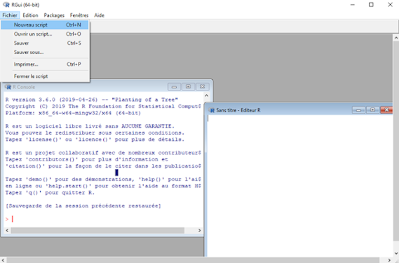
\includegraphics{images/screenshotR.png}

\begin{itemize}
\tightlist
\item
  Un IDE, \emph{Integrated Development Environment}: un editor de
  scripts - es un entorno mucho más amigable que facilita el trabajo
  (gestión de archivos, objetos y comandos, historial de funciones,
  autocompletado,\ldots)
\item
  El IDE más utilizado es \textbf{RStudio} (pero hay otros como
  \textbf{Tinn-R} o \textbf{jamovi}).
\item
  Los comandos y funciones son los mismos para \textbf{R} y
  \textbf{RStudio}.
\end{itemize}

\hypertarget{instalaciuxf3n}{%
\subsection{Instalación}\label{instalaciuxf3n}}

\begin{enumerate}
\def\labelenumi{\arabic{enumi}.}
\item
  Descargar e instalar \href{https://cran.r-project.org/}{\textbf{R
  básico}} - Elija su sistema operativo y siga los pasos.
\item
  Descargar e instalar
  \href{https://www.rstudio.com/products/rstudio/download/\#download}{\textbf{RStudio}}
  (u otra interfaz) - Elija la versión gratuita y su sistema operativo.
\item
  Verificar si tienes los paquetes (\emph{package}): \emph{rmarkdown} y
  \emph{knitr} en \textbf{RStudio}:
\end{enumerate}

En la consola de R, utilizar lo siguiente:

\begin{Shaded}
\begin{Highlighting}[]
\FunctionTok{find.package}\NormalTok{(}\FunctionTok{c}\NormalTok{(}\StringTok{"rmarkdown"}\NormalTok{,}\StringTok{"knitr"}\NormalTok{))}
\end{Highlighting}
\end{Shaded}

\begin{verbatim}
## [1] "C:/Users/EvelynG/Documents/R/win-library/4.0/rmarkdown"
## [2] "C:/Users/EvelynG/Documents/R/win-library/4.0/knitr"
\end{verbatim}

Si no lo tiene, puedes instalarlos con los siguiente comandos.

En la consola de R, utilizar lo siguiente:

\begin{Shaded}
\begin{Highlighting}[]
\FunctionTok{install.packages}\NormalTok{(}\StringTok{"rmarkdown"}\NormalTok{)}
\FunctionTok{install.packages}\NormalTok{(}\StringTok{"knitr"}\NormalTok{)}
\end{Highlighting}
\end{Shaded}

\hypertarget{quuxe9-es-un-paquete-o-package}{%
\subsubsection{\texorpdfstring{¿Qué es un paquete o
\emph{package}?}{¿Qué es un paquete o package?}}\label{quuxe9-es-un-paquete-o-package}}

\begin{itemize}
\item
  Un \emph{paquete} es un módulo (o extensión, biblioteca) que contiene
  un conjunto de funciones (a menudo relacionadas con un método o
  dominio particular)
\item
  En la instalación, \textbf{R} viene con un conjunto de funciones
  básicas \{base\} y módulos por defecto (\emph{built-in packages}).
\item
  La comunidad desarrolla constantemente \emph{paquetes} de funciones
  especializadas.
\item
  Hay más de 15.000 en el sitio web oficial de \textbf{R}
  \href{https://cran.r-project.org/web/packages/}{CRAN}. También se
  pueden encontrar otros en otros lugares (Github, por ejemplo).
\item
  Los paquetes deben ser \textbf{descargados}
  (\texttt{install.packages()} o pueden ser instalados a través del menú
  superior de RStudio \emph{Tools\textgreater Install
  packages\ldots{}}). Solo es necesario instalarlos una vez; sin
  embargo, se deberán \textbf{cargar} (\texttt{library()} o
  \texttt{require()}) cada sesión que se quieran utilizar.
\item
  Una función (por ejemplo, correlación, tablas de contingencia\ldots)
  puede encontrarse en varios paquetes con variantes más o menos
  importantes (procedimientos, opciones, argumentos, resultados).
\item
  Los paquetes también deben actualizarse periódicamente. Esto se puede
  realizar a través de: \emph{Tools\textgreater Check for package
  updates\ldots{}}.
\end{itemize}

\hypertarget{fundamentos-rmarkdown}{%
\section{Fundamentos RMarkdown}\label{fundamentos-rmarkdown}}

\hypertarget{motivaciuxf3n---ejemplos-rmd}{%
\subsection{Motivación - Ejemplos
Rmd}\label{motivaciuxf3n---ejemplos-rmd}}

Multiples opciones de publicaciones con RMarkdown:

\begin{itemize}
\tightlist
\item
  Esta página web.
\item
  Repositorio de conocimientos
  \href{https://www.tandfonline.com/doi/full/10.1080/00031305.2017.1392362?journalCode=utas20}{Aibnb.}
\item
  Tareas académicas en \href{https://rpubs.com/}{Rpubs}.
\item
  Correos personalizados
  \href{https://rmarkdown.rstudio.com/articles_mail_merge.html}{Mine
  Çetinkaya-Rundel}.
\item
  Encuesta sobre beneficios de salud para empleadores de
  \href{https://www.kff.org/health-costs/report/2017-employer-health-benefits-survey/}{2017.}
\item
  Dashboards en
  \href{https://www.eelloo.nl/wp-content/uploads/2017/08/infographic_Voorbeelden-infographics-Overzicht.pdf}{eelloo}.
\end{itemize}

\hypertarget{quuxe9-es-r-markdown}{%
\subsection{¿Qué es R Markdown ?}\label{quuxe9-es-r-markdown}}

\begin{quote}
R + Markdown = RMarkdown
\end{quote}

\begin{itemize}
\item
  R Markdown es un paquete instalado por defecto en RStudio.
\item
  Es una herramienta creada para asegurar la \textbf{reproducibilidad}
  de un análisis o una investigación integrando en un único documento el
  texto en Markdown, el código (R u otro) y los resultados de su
  análisis.
\item
  Evita todos los pasos de copiar y pegar tablas, gráficos, imágees, y
  crea documentos o presentaciones fáciles de actualizar en diferentes
  formatos: word, pdf, ppt, html, etc.
\item
  Está optimizado para la creación de documentos html (formato que se
  beneficia de las opciones más interesantes).
\end{itemize}

\hypertarget{beneficios-de-usar-rmarkdown}{%
\subsection{Beneficios de usar
RMarkdown}\label{beneficios-de-usar-rmarkdown}}

Los beneficios de usar RMarkdown:

\begin{itemize}
\tightlist
\item
  Simple y sencillo: Crear contenido web es rápido y cómodo.
\item
  A prueba de errores: Difícil cometer errores de sintaxis.
\item
  Minimalista: Es perfecto para usarlo con editores de texto
  minimalistas.
\item
  Versátil: Permite desarrollar análisis de datos y redactar un informe
  a la vez.
\end{itemize}

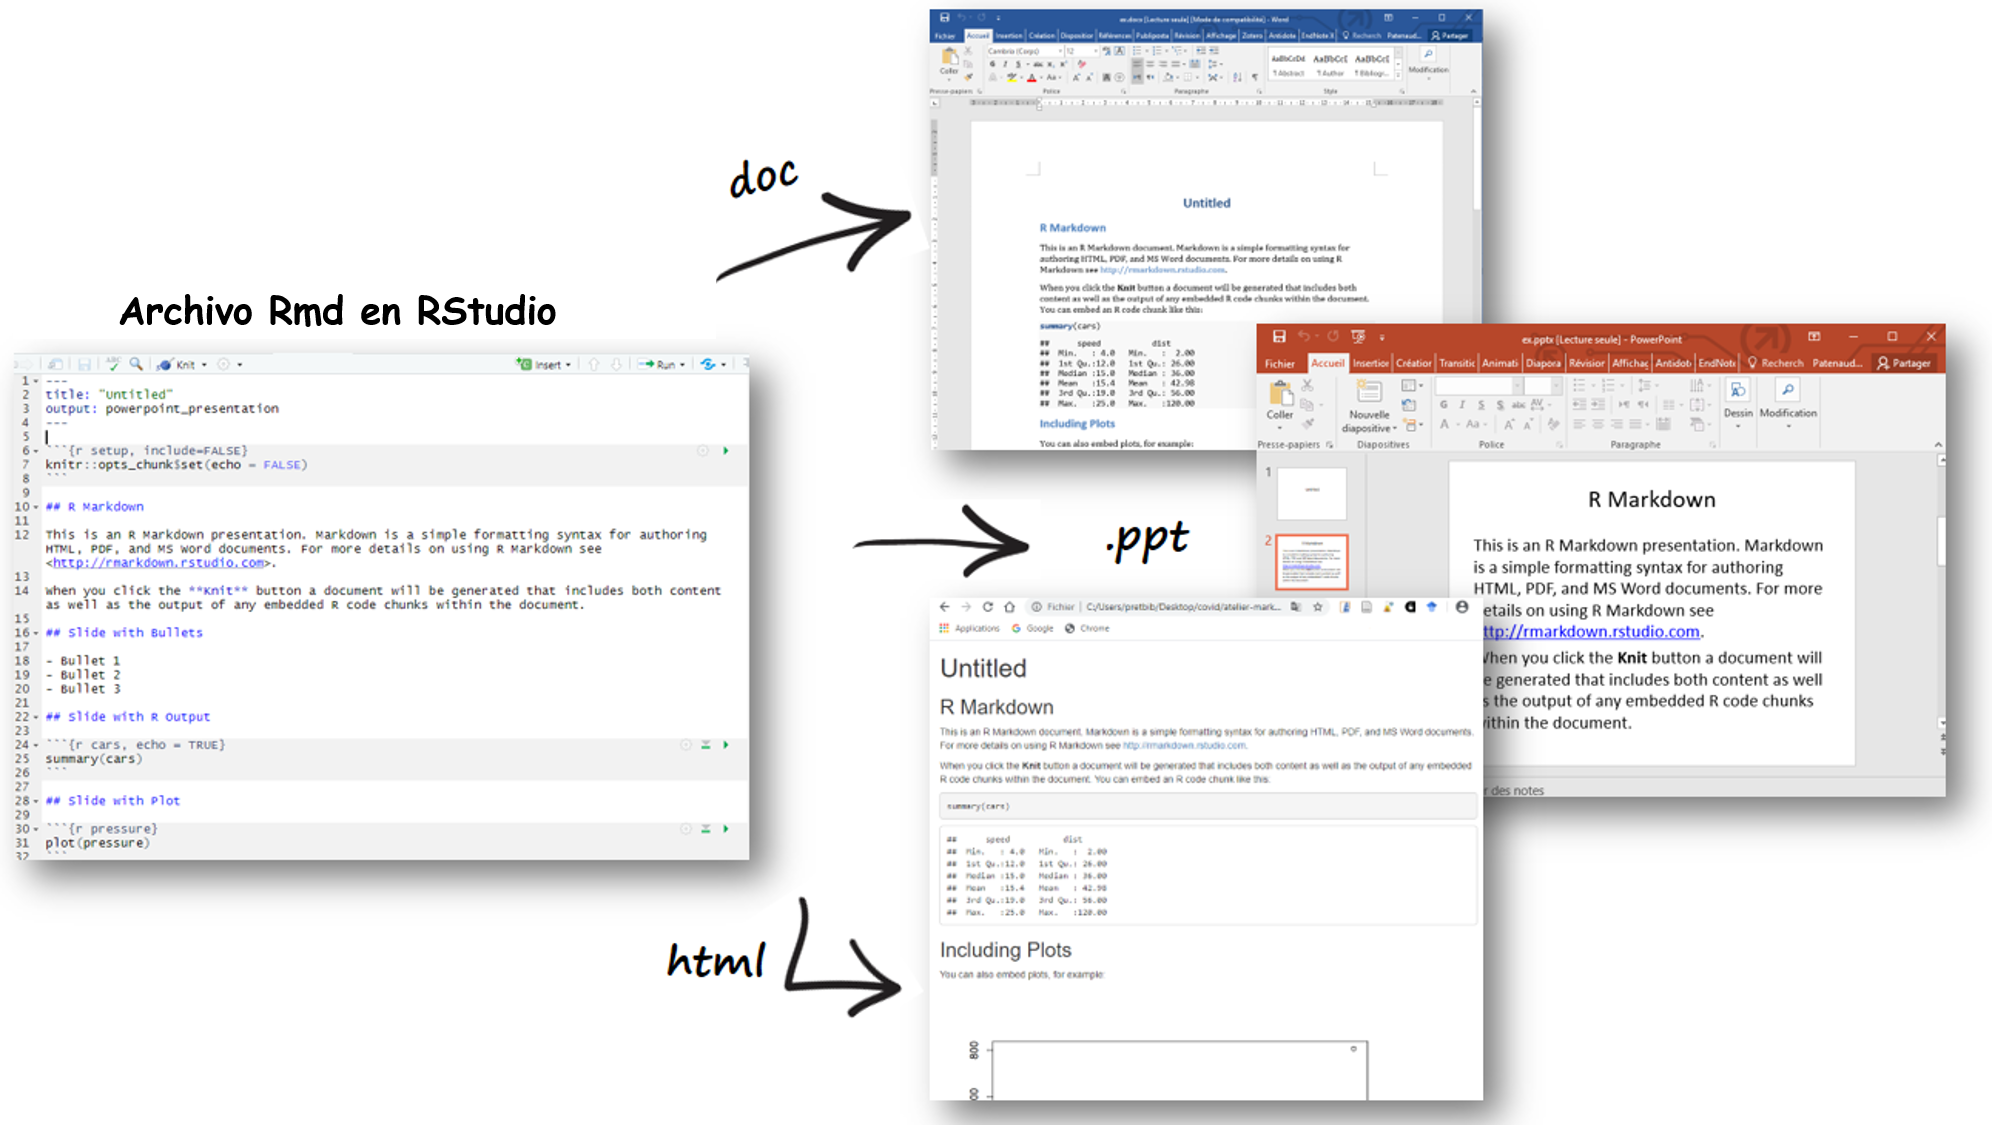
\includegraphics[width=0.8\textwidth,height=\textheight]{images/formatexport.png}

\hypertarget{cuxf3mo-funciona}{%
\subsection{¿Cómo funciona?}\label{cuxf3mo-funciona}}

R Markdown combina diferentes procesos para crear documentos en
diferentes formatos a partir de un único archivo:

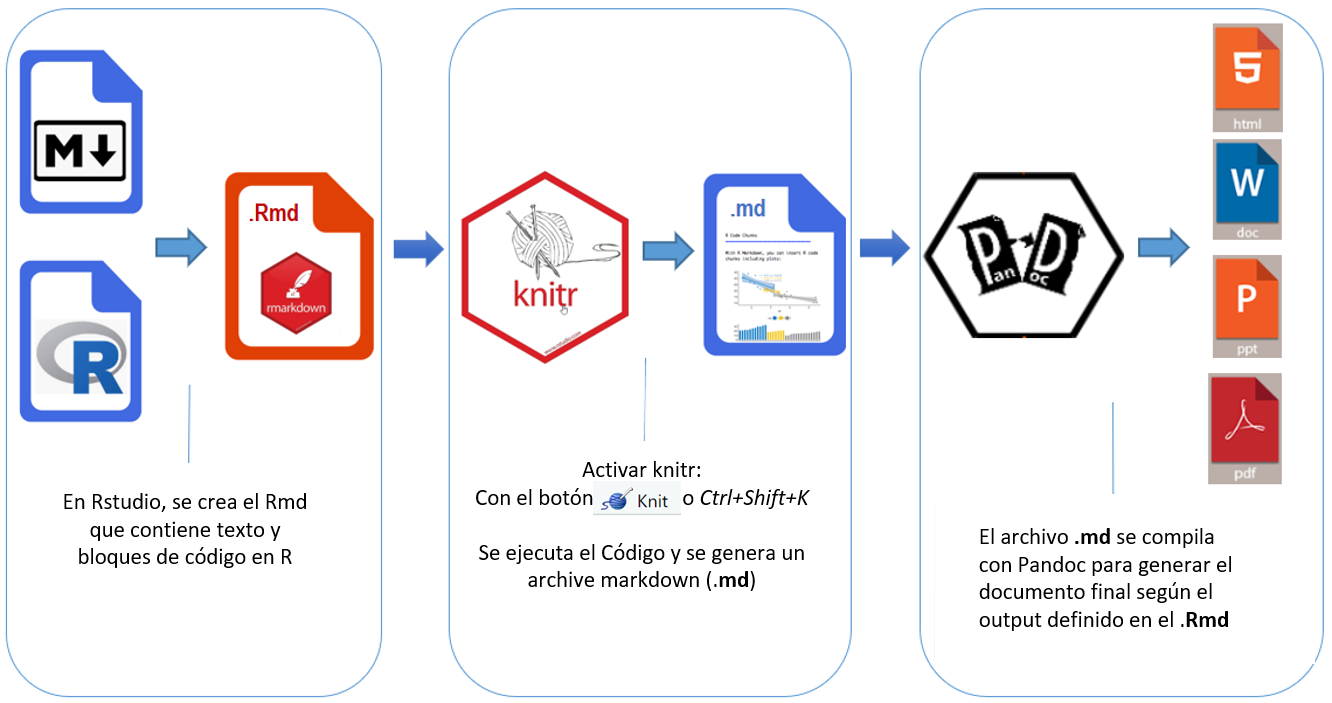
\includegraphics[width=0.75\textwidth,height=\textheight]{images/workflow.png}

\begin{itemize}
\item
  Todo comienza con la creación de un documento \textbf{.Rmd} en
  RStudio. Un archivo R Markdown es un simple archivo de texto con una
  extensión .Rmd (puede crearlo en el Bloc de notas).
\item
  Para generar un reporte, en RStudio utilice el botón knit que activa
  la función \texttt{rmarkdown::render()} y ejecuta los bloques de
  código en el archivo \textbf{.Rmd} para incluirlos en el documento
  final. Estos resultados se convierten en un archivo temporal .md (que
  contiene el código y los resultados).
\item
  Este es un bloque de código para compilar un documento y establecer el
  formato de salida con el argumento \emph{output\_format} de la función
  \texttt{render}:
\end{itemize}

\begin{Shaded}
\begin{Highlighting}[]
\FunctionTok{library}\NormalTok{(rmarkdown)}
\FunctionTok{render}\NormalTok{(}\StringTok{"1{-}example.Rmd"}\NormalTok{, }\AttributeTok{output\_format =} \StringTok{"word\_document"}\NormalTok{) }
\end{Highlighting}
\end{Shaded}

\begin{itemize}
\item
  A continuación, este archivo \textbf{.md} es procesado por la
  herramienta \emph{Pandoc}, que permite convertir el contenido de un
  lenguaje de marcas (\emph{markup}) en diferentes formatos (``navaja
  suiza'' de la conversión de formatos de documentos). Los parámetros de
  conversión se especifican en la cabecera \textbf{YAML} del documento
  \textbf{.Rmd}, donde entre otras cosas se especifica el formato final.
\item
  Si el formato final deseado es pdf, se añade un paso de procesamiento
  adicional: \emph{Pandoc} transformará el archivo \textbf{.md} en otro
  archivo intermedio .tex. Este archivo .tex será luego procesado por
  \emph{LaTeX} en su forma final de pdf.
\end{itemize}

\hypertarget{cuxf3mo-creo-un-nuevo-rmd}{%
\subsection*{¿Cómo creo un nuevo Rmd?}\label{cuxf3mo-creo-un-nuevo-rmd}}
\addcontentsline{toc}{subsection}{¿Cómo creo un nuevo Rmd?}

Creación de un Rmd en RStudio 🐣:

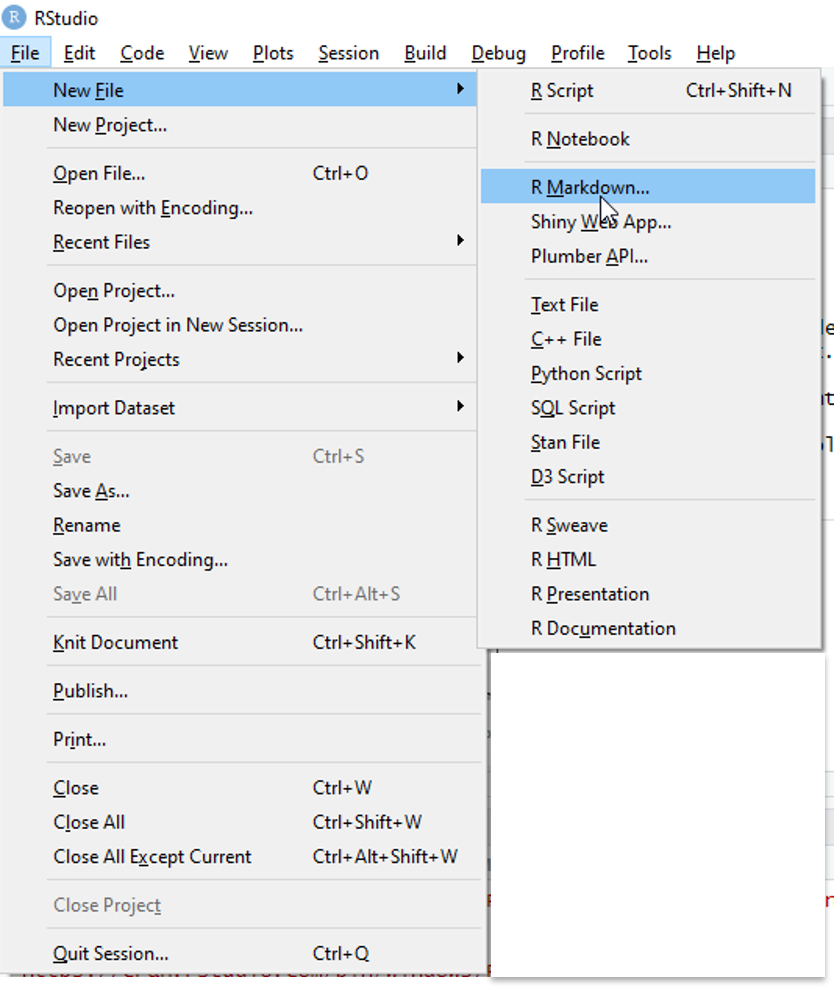
\includegraphics[width=0.4\textwidth,height=\textheight]{images/crear_mkd.png}

👩‍💻 👨‍💻 Ejercicio 1: Crear y compilar un Rmd

\hypertarget{formatos-de-salida}{%
\section{Formatos de salida}\label{formatos-de-salida}}

\hypertarget{formatos-buxe1sicos}{%
\subsection{Formatos básicos}\label{formatos-buxe1sicos}}

\begin{enumerate}
\def\labelenumi{\arabic{enumi}.}
\tightlist
\item
  \textbf{Formatos de documentos:}

  \begin{itemize}
  \tightlist
  \item
    html\_document
  \item
    odt\_document
  \item
    rtf\_document
  \item
    word\_document
  \item
    github\_document
  \item
    md\_document
  \item
    pdf\_document (LaTeX/pdf)
  \item
    latex\_document (LaTeX/pdf)
  \item
    beamer\_presentation (LaTeX/pdf)
  \end{itemize}
\item
  \textbf{Formatos de presentación:}

  \begin{itemize}
  \tightlist
  \item
    ioslides\_presentation (\emph{slides html})
  \item
    slidy\_presentation (\emph{slides html})
  \item
    revealjs::revealjs\_presentation (\emph{slides html + js})
  \item
    powerpoint\_presentation
  \end{itemize}
\end{enumerate}

\textbf{Opcional:} Para crear archivos PDF utilizando RMarkdown,
necesitaremos tener instalado una distribución de LaTeX. Si no tienes
instalado LateX, recomendamos instalar
\href{https://yihui.org/tinytex/}{TinyTeX}.

En la consola de R, utilizar lo siguiente:

\begin{Shaded}
\begin{Highlighting}[]
\FunctionTok{install.packages}\NormalTok{(}\StringTok{\textquotesingle{}tinytex\textquotesingle{}}\NormalTok{)}
\NormalTok{tinytex}\SpecialCharTok{::}\FunctionTok{install\_tinytex}\NormalTok{()  }\CommentTok{\# Instala TinyTeX}
\end{Highlighting}
\end{Shaded}

TinyTex es una distribución ligera de LaTex. Sin embargo, esta
instalación podría demorar según tu conexión a internet.

\hypertarget{otros-formatos---plantillas}{%
\subsection{Otros formatos -
Plantillas}\label{otros-formatos---plantillas}}

Hay un gran número de \emph{paquetes} y \emph{plantillas} para crear
diferentes tipos de documentos con una amplia variedad de estilos
predefinidos: plantillas de presentación, artículos periodísticos,
libros, tesis, sitios web, blogs, widgets, cuadros de mando, mapas y
otras presentaciones interactivas\ldots{}

\begin{itemize}
\item
  Ver \href{https://rmarkdown.rstudio.com/gallery.html}{galeria}
\item
  Algunos de los más conocidos:

  \begin{itemize}
  \tightlist
  \item
    \href{https://github.com/yixuan/prettydoc/}{prettydoc}
  \item
    \href{https://bookdown.org/yihui/bookdown/}{bookdown}
  \item
    \href{https://bookdown.org/yihui/blogdown/}{blogdown}
  \item
    \href{https://github.com/rstudio/distill}{distill}
  \item
    \href{https://bookdown.org/yihui/rmarkdown/xaringan-format.html}{xaringan}
  \item
    \href{https://rmarkdown.rstudio.com/flexdashboard/}{flexdashboard}
  \item
    \href{http://mangothecat.github.io/rmdshower/skeleton.html}{rmdshower}
  \item
    \href{https://github.com/mitchelloharawild/vitae}{vitae}
  \end{itemize}
\item
  Hay que tener en cuenta que el uso de estas diferentes herramientas
  requiere el aprendizaje de una configuración/etiquetado particular que
  puede ir en detrimento de la interoperabilidad de los formatos.
\item
  También puede crear sus propias
  \href{https://rstudio.github.io/rstudio-extensions/rmarkdown_templates.html}{plantillas}
  y
  \href{https://bookdown.org/yihui/rmarkdown/word-document.html}{estilo
  de documento}
\end{itemize}

👩‍💻 👨‍💻 Ejercicio 2: añadir un tema de
\href{https://github.com/yixuan/prettydoc/}{prettydoc} al Rmd.

\hypertarget{estructura-de-un-documento-rmarkdown}{%
\section{Estructura de un documento
RMarkdown}\label{estructura-de-un-documento-rmarkdown}}

\hypertarget{partes}{%
\subsection{Partes}\label{partes}}

Contiene 3 partes:

\begin{enumerate}
\def\labelenumi{\arabic{enumi}.}
\tightlist
\item
  Un encabezado de metadatos (\emph{encabezado YAML}): encabezado
  escrito en \href{https://en.wikipedia.org/wiki/YAML}{\textbf{YAML}}
  rodeado por 3 guiones.
\item
  Texto: formateado en markdown.
\item
  Bloques de código: \emph{códigos} encerrados entre triple tilde
  invertida (acentos agudos) ```` (Para crearlos rapidamente se puede
  usar \emph{ctrl +alt + i}).
\end{enumerate}

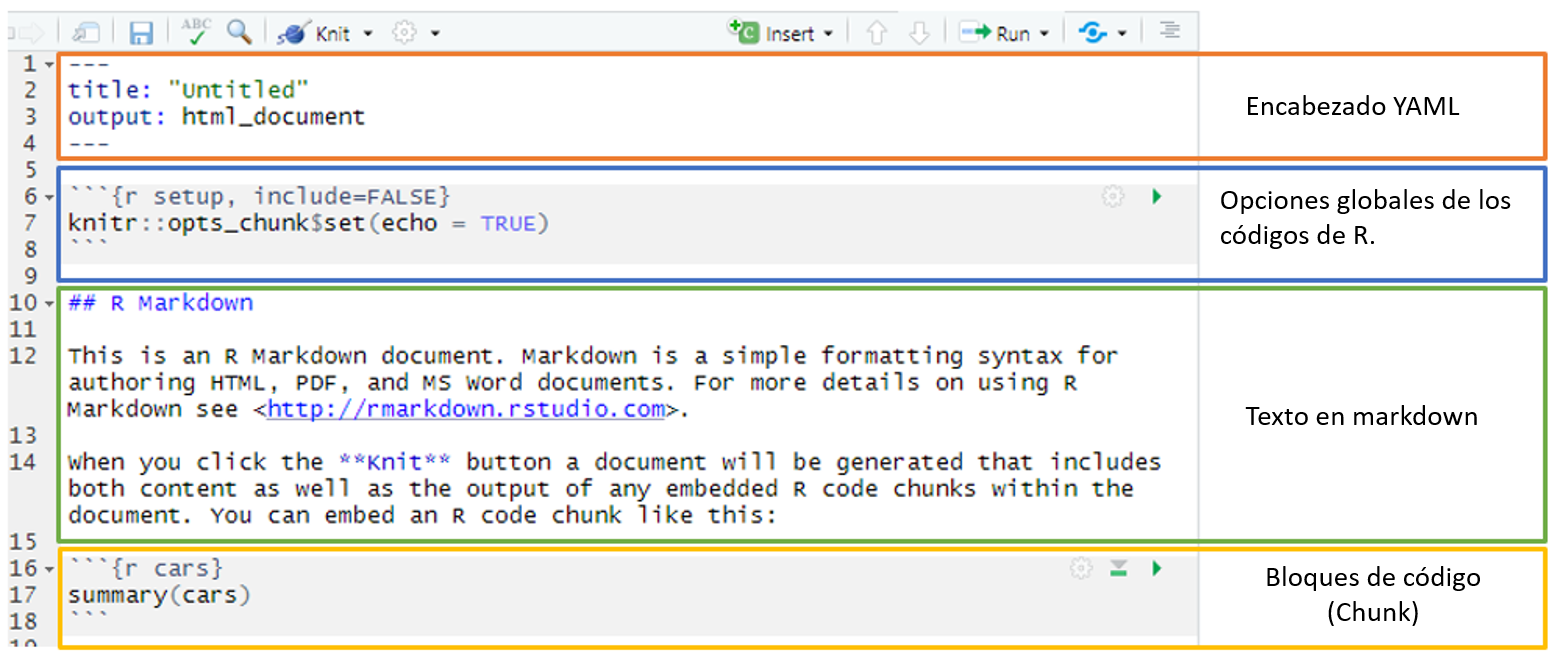
\includegraphics[width=0.75\textwidth,height=\textheight]{images/estructura.png}

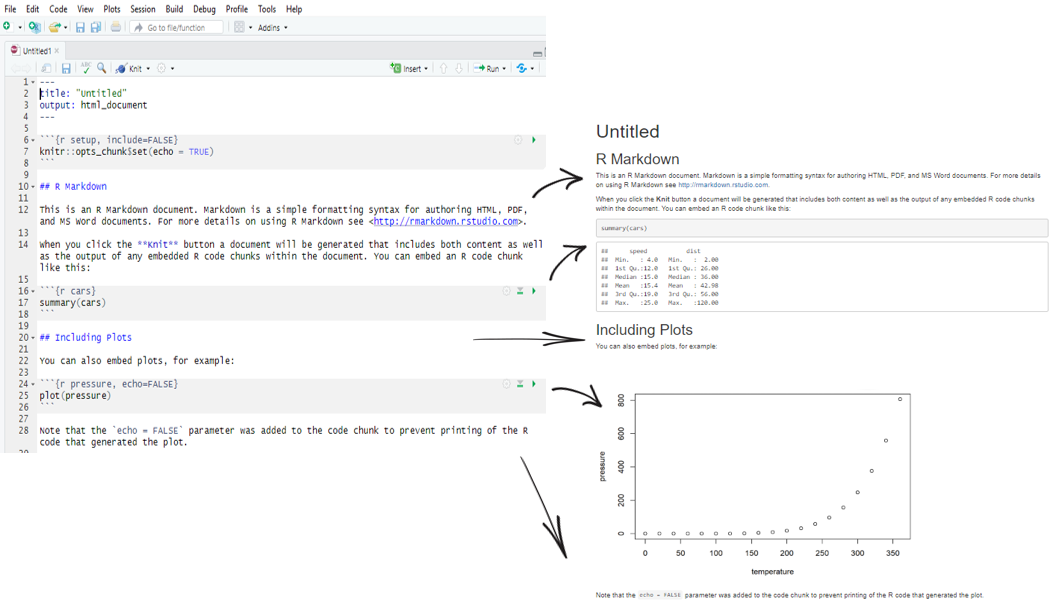
\includegraphics[width=0.85\textwidth,height=\textheight]{images/bloques.png}

\hypertarget{metadatos}{%
\subsection{Metadatos}\label{metadatos}}

\begin{itemize}
\tightlist
\item
  Metadatos básicos y campos de Ouput para definir el formato y sus
  opciones para configurar la presentación final
\item
  Sintaxis \href{https://en.wikipedia.org/wiki/YAML}{YAML}
\end{itemize}

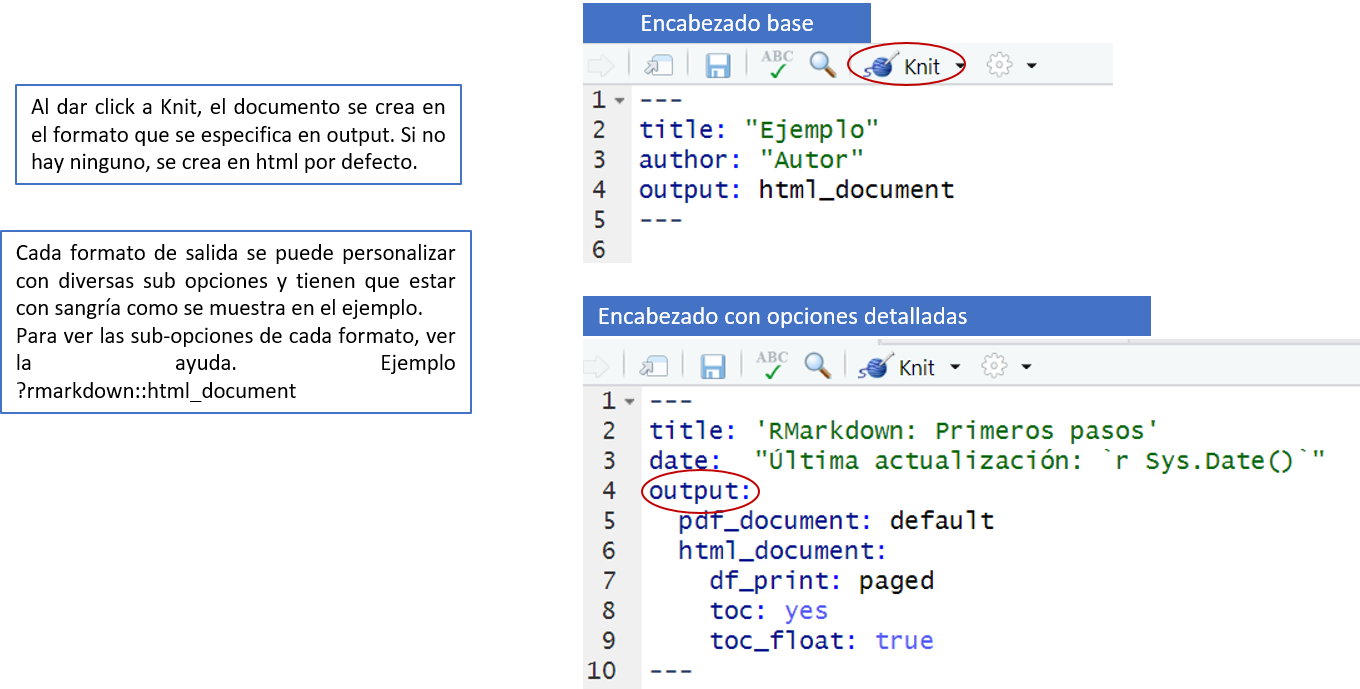
\includegraphics[width=0.7\textwidth,height=\textheight]{images/yaml_ejemplo.png}

\begin{itemize}
\tightlist
\item
  Cada \href{https://rmarkdown.rstudio.com/formats.html}{formato de
  salida} tiene opciones específicas para personalizar la presentación
  final con argumentos como subvalores del campo \emph{output}: (las
  subopciones deben estar con sangría).
\item
  Para saber cuáles son estas opciones, consultar la ayuda:
  \texttt{?rmarkdown::html\_document}.
\item
  Si un formato de salida es proporcionado por un paquete en específico,
  debe ser nombrado en el campo YAML
  \texttt{output:\ tufte::tufte\_html}.
\end{itemize}

\hypertarget{editar-metadatos}{%
\subsection{Editar metadatos}\label{editar-metadatos}}

También es posible controlar el formato del documento final utilizando
las opciones del menú \textbf{knit} de RStudio. El encabezado YAML se
modificarán automáticamente.

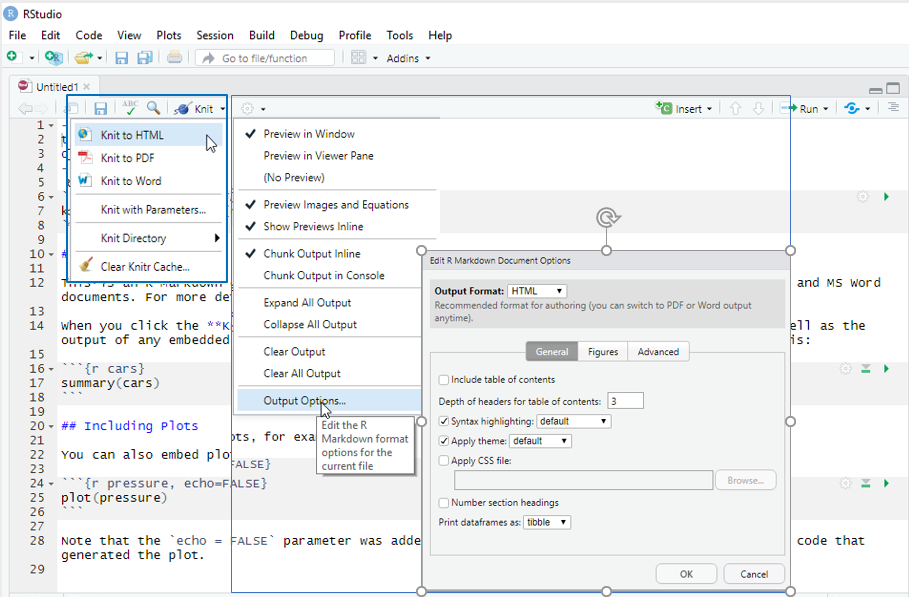
\includegraphics{images/options.png}

\hypertarget{markdown}{%
\section{Markdown}\label{markdown}}

\hypertarget{conocer-markdown.}{%
\subsection{Conocer Markdown.}\label{conocer-markdown.}}

\begin{itemize}
\item
  \href{https://daringfireball.net/projects/markdown/syntax}{Markdown}
  es un lenguaje de marcado, una versión simplificada de html, creado
  por John Gruber en 2004.
\item
  Se utiliza para estructurar contenidos textuales y producir documentos
  a partir de texto plano etiquetado.
\end{itemize}

\begin{quote}
Markdown refleja la filosofía del estoicismo: el ``mundo natural''
consiste en texto plano, y no hay que dejarse controlar por el deseo de
placer (visual). ---
\href{https://bookdown.org/yihui/rmarkdown-cookbook/formatting.html}{Yihui}
\end{quote}

\begin{itemize}
\item
  A menudo se compara con \href{https://www.latex-project.org/}{LaTeX};
  otro lenguaje de marcado más potente pero mucho más complejo para
  producir documentos pdf.
\item
  Existen varias versiones de Markdown desarrolladas por diferentes
  programadores. La que utiliza
  \href{https://rmarkdown.rstudio.com/authoring_pandoc_markdown.html\%23raw-tex\#pandoc_markdown}{R
  Markdown} es la versión de
  \href{https://pandoc.org/MANUAL.html}{Pandoc} que también permite
  convertir los documentos en diferentes formatos.
\item
  Su gran sencillez lo convierte en una herramienta más limitada en
  cuanto a la estructuración de documentos que el html, LaTeX y los
  programas de tratamiento de textos.
  (\href{https://daringfireball.net/projects/markdown/syntax\#philosophy}{Ver
  Gruber (Creador de )})
\item
  Por lo tanto, es útil conocer estos lenguajes (html, css, javascript,
  LaTeX) si quiere personalizar el formato de sus documentos (pero tenga
  cuidado porque el uso de html y LaTeX puede causar problemas al
  exportar a ciertos formatos).
\end{itemize}

\hypertarget{sintaxis-buxe1sica-de-markdown}{%
\subsection{Sintaxis básica de
Markdown}\label{sintaxis-buxe1sica-de-markdown}}

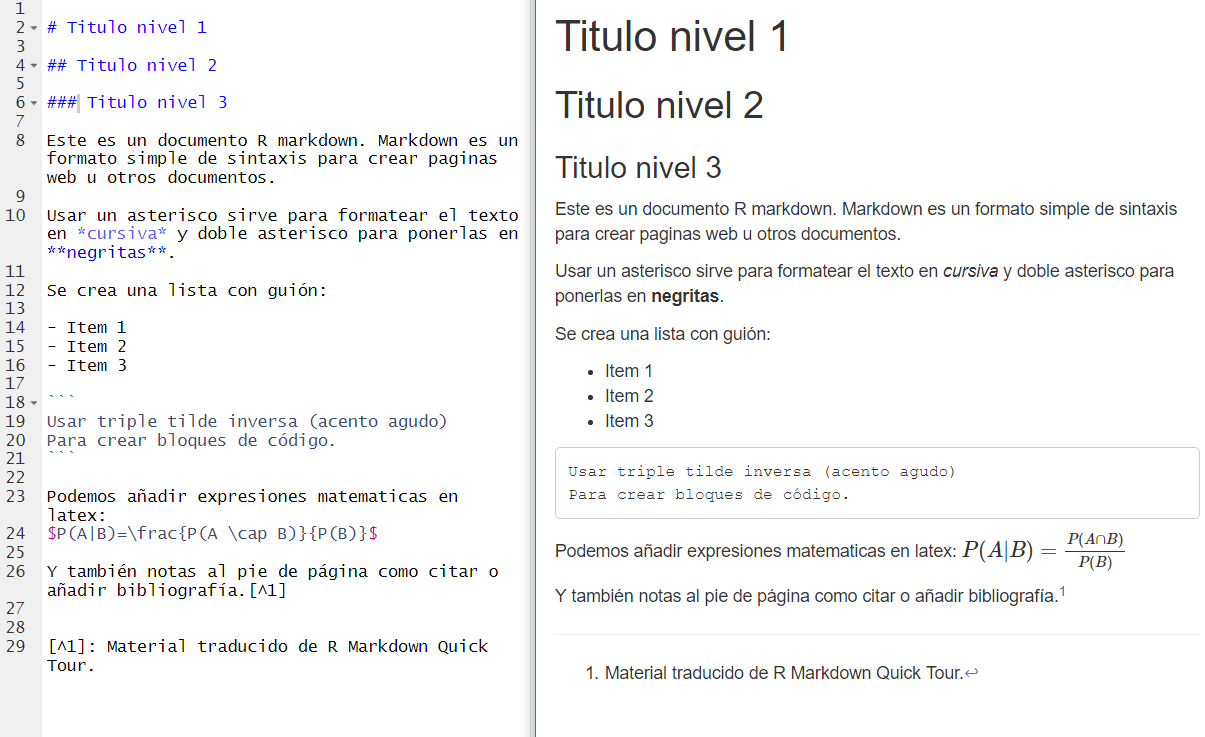
\includegraphics{images/Markdown_ejemplo.PNG}

\href{ejemplos/ejemplo_markdown.Rmd}{Descargar muestra}

\href{https://rstudio.com/wp-content/uploads/2015/03/rmarkdown-reference.pdf}{Guía
de referencia}

\href{https://www.markdowntutorial.com/}{Tutorial de Markdown}

\hypertarget{formato}{%
\subsection{Formatear texto.}\label{formato}}

\hypertarget{negrita-y-cursiva}{%
\subsubsection{Negrita y Cursiva}\label{negrita-y-cursiva}}

Podemos utilizar algunos símbolos alrededor de nuestro texto para
resaltarlo con negrita o cursiva:

Poner \texttt{*} entre el texto cambiará el estilo del texto a cursiva
mientras que \texttt{**} cambiará nuestro texto a negritas:

\begin{longtable}[]{@{}lc@{}}
\toprule
En Rmd: & Resultado \\
\midrule
\endhead
\texttt{*Cursiva*} & \emph{Cursiva} \\
\texttt{**Negrita**} & \textbf{Negrita} \\
\bottomrule
\end{longtable}

\hypertarget{otros-elementos}{%
\subsubsection{Otros elementos:}\label{otros-elementos}}

Algunas otras opciones de personalización de texto incluyen los
siguientes elementos:

\begin{longtable}[]{@{}lll@{}}
\toprule
Elemento & En Rmd: & Resultado \\
\midrule
\endhead
Subindice & \texttt{H\textasciitilde{}2\textasciitilde{}O} &
H\textsubscript{2}O \\
Superindice & \texttt{E=mc\^{}2\^{}} & E=mc\textsuperscript{2} \\
\bottomrule
\end{longtable}

\begin{longtable}[]{@{}lcl@{}}
\toprule
Elem. & En Rmd: & Resultado \\
\midrule
\endhead
URL & \texttt{{[}FIEECS{]}(https://fieecs.uni.edu.pe/)} &
\href{https://fieecs.uni.edu.pe/}{FIEECS} \\
Imagen & \texttt{!{[}RStudio{]}(RStudio-icon.png)} &

\includegraphics[width=0.20833in,height=\textheight]{img/RStudio-icon.png} \\
\bottomrule
\end{longtable}

\hypertarget{niveles}{%
\subsection{Diferentes niveles de texto.}\label{niveles}}

\hypertarget{sec}{%
\subsubsection{Secciones}\label{sec}}

Para crear titulos, utilizamos \texttt{\#} al inicio del texto:

\texttt{\#\ Encabezado\ de\ primer\ nivel\ \{-\}}~\\
\texttt{\#\#\ Encabezado\ de\ segundo\ nivel}~\\
\texttt{\#\#\#\ Encabezado\ de\ tercer\ nivel}~\\

\begin{center}\rule{0.5\linewidth}{0.5pt}\end{center}

\hypertarget{listas}{%
\subsubsection{Crear listas}\label{listas}}

Utilizando el siguiente código:

\texttt{1.\ Primer\ item}~\\
\texttt{2.\ Segundo\ item}~\\
\texttt{3.\ Tercer\ item}~\\
\texttt{-\ un\ item\ sin\ numeración}~\\
\texttt{-\ otro\ item\ sin\ numeración}~\\

Obtenemos lo siguiente:

\begin{enumerate}
\def\labelenumi{\arabic{enumi}.}
\tightlist
\item
  Primer item.
\item
  Segundo item.
\item
  Tercer item.

  \begin{itemize}
  \tightlist
  \item
    un item sin numeración.
  \item
    otro item sin numeración.
  \end{itemize}
\end{enumerate}

\begin{center}\rule{0.5\linewidth}{0.5pt}\end{center}

\hypertarget{expre}{%
\subsection{Expresiones matemáticas}\label{expre}}

Para comenzar a utilizar la sintaxis de LaTeX dentro de un Rmd,
utilizamos \texttt{\$} y \texttt{\$\$}. Si deseamos escribir expresiones
dentro de una línea de texto, usamos \texttt{\$}, y para expresiones
matemáticas en un nuevo párrafo usamos \texttt{\$\$}

Ejemplos:

Al utilizar el siguiente código (copiar y pegar el código en un Rmd).

\texttt{\$\$f(k)\ =\ \{n\ \textbackslash{}choose\ k\}\ p\^{}\{k\}\ (1-p)\^{}\{n-k\}\$\$}

Se obtendrá el siguiente resultado:

\[f(k) = {n \choose k} p^{k} (1-p)^{n-k}\]

Más sobre expresiones matemáticas en la
\href{https://bookdown.org/yihui/rmarkdown/markdown-syntax.html\#math-expressions}{guía
oficial}

👩‍💻 👨‍💻 Ejercicio: Crear un modelo de reporte con las secciones que
debes tener para un análisis exploratorio. Por ejemplo: Lectura de
datos, Análisis exploratorio univariado, y análisis exploratorio
multivariado. Puedes ser creativo con los nombres. Además, añadir los
siguientes elementos:

\begin{itemize}
\tightlist
\item
  Negritas y cursivas.
\item
  Añadir logo.
\item
  Añadir imagen de RStudio.
\end{itemize}

\href{ejemplos/ejemplo_markdown_sintax_guiaPrimerosPasos.Rmd}{Ejemplo de
Rmd con sintaxis markdown}

\hypertarget{cuxf3digos-de-r-chunks}{%
\section{Códigos de R (Chunks)}\label{cuxf3digos-de-r-chunks}}

El código R puede incluirse de dos maneras:

\begin{enumerate}
\def\labelenumi{\arabic{enumi}.}
\tightlist
\item
  \textbf{En bloques de código} (\emph{chunks}): inician con ```\{r\}
  (donde r indique el lenguaje a utilizar, y se puede poner otros como:
  python, sql, \ldots)
\end{enumerate}

\begin{Shaded}
\begin{Highlighting}[]
\InformationTok{\textasciigrave{}\textasciigrave{}\textasciigrave{}\{r\}}
\InformationTok{mean(23, 65, 43, 34, 56) \# El estilo de los bloques se define mediante la opción "highlight" en el YAML}
\InformationTok{\textasciigrave{}\textasciigrave{}\textasciigrave{}}
\end{Highlighting}
\end{Shaded}

\begin{itemize}
\tightlist
\item
  Las etiquetas de bloque se pueden añadir con el botón \emph{insert} o
  con \emph{Ctrl + Alt + i}.
\item
  Lo mejor es dividir el código que genera diferentes salidas en
  diferentes bloques
\end{itemize}

\begin{enumerate}
\def\labelenumi{\arabic{enumi}.}
\setcounter{enumi}{1}
\tightlist
\item
  \textbf{En el texto} (\emph{Inline R code}) que comienza con
  \texttt{r} y termina con un acento
  \texttt{\textasciigrave{}\textasciigrave{}}.
\end{enumerate}

\textbf{Código: }

\begin{Shaded}
\begin{Highlighting}[]
\NormalTok{La edad media de nuestros participantes es }\InformationTok{\textasciigrave{}r mean(23, 65, 21, 22, 26)\textasciigrave{}}
\end{Highlighting}
\end{Shaded}

\textbf{Resultados}:

La edad media de nuestros participantes es 23.

\hypertarget{ejemplo-diamantes}{%
\subsection{Ejemplo: diamantes}\label{ejemplo-diamantes}}

\textbf{Texto Markdown}

\begin{Shaded}
\begin{Highlighting}[]
\CommentTok{{-}{-}{-}}
\AnnotationTok{title:}\CommentTok{ "Diamantes"}
\AnnotationTok{date:}\CommentTok{ 2021{-}08{-}21  \#o usar Sys.Date()}
\AnnotationTok{output:}\CommentTok{ html\_document}
\CommentTok{{-}{-}{-}}

\InformationTok{\textasciigrave{}\textasciigrave{}\textasciigrave{}\{r setup, include = FALSE\}}
\InformationTok{library(ggplot2)}
\InformationTok{library(dplyr)}

\InformationTok{smaller \textless{}{-} diamonds \%\textgreater{}\% }
\InformationTok{  filter(carat \textless{}= 2.5)}
\InformationTok{\textasciigrave{}\textasciigrave{}\textasciigrave{}}

\NormalTok{Tenemos }\InformationTok{\textasciigrave{}r nrow(diamonds)\textasciigrave{}}\NormalTok{ diamantes. Solo }
\InformationTok{\textasciigrave{}r nrow(diamonds) {-} nrow(smaller)\textasciigrave{}}\NormalTok{ pesan más de }
\KeywordTok{\textless{}span}\OtherTok{ style=}\StringTok{"color:red"}\KeywordTok{\textgreater{}}\NormalTok{ 2.5 quilates }\KeywordTok{\textless{}/span\textgreater{}}\NormalTok{. La distribución del resto es la siguiente:}

\InformationTok{\textasciigrave{}\textasciigrave{}\textasciigrave{}\{r, echo = FALSE\}}
\InformationTok{smaller \%\textgreater{}\% }
\InformationTok{  ggplot(aes(carat)) + }
\InformationTok{  geom\_freqpoly(binwidth = 0.1)}
\InformationTok{\textasciigrave{}\textasciigrave{}\textasciigrave{}}
 
\end{Highlighting}
\end{Shaded}

\textbf{Output}

\begin{verbatim}
## PhantomJS not found. You can install it with webshot::install_phantomjs(). If it is installed, please make sure the phantomjs executable can be found via the PATH variable.
\end{verbatim}

\hypertarget{configuraciuxf3n-de-chunks.}{%
\subsection{\texorpdfstring{Configuración de
\emph{chunks}.}{Configuración de chunks.}}\label{configuraciuxf3n-de-chunks.}}

\begin{itemize}
\item
  El ``comportamiento'' de los bloques de código y la presentación de
  los resultados pueden configurarse de varias maneras.
\item
  Knitr ofrece muchas
  \href{https://rstudio.com/wp-content/uploads/2015/03/rmarkdown-reference.pdf}{opciones}
  (\emph{chunck options}) que pueden añadirse como argumentos entre las
  llaves de cada bloque (cada opción debe estar separada por una coma).
\end{itemize}

\begin{Shaded}
\begin{Highlighting}[]
\InformationTok{\textasciigrave{}\textasciigrave{}\textasciigrave{}\{r, chunk{-}label, results=\textquotesingle{}hide\textquotesingle{}, fig.height=4\}}
\InformationTok{\textasciigrave{}\textasciigrave{}\textasciigrave{}}
\end{Highlighting}
\end{Shaded}

\begin{itemize}
\item
  Cada bloque puede tener opcionalmente un nombre (\emph{etiqueta}),
  debe ser la primera opción.
\item
  Estas opciones controlan esencialmente cómo se compila (o no) el
  código de cada bloque y cómo se presentan (o no) los resultados de
  cada bloque de código.
\item
  Muchos de los argumentos tienen valores lógicos: TRUE O FALSE (con un
  valor por defecto que debe ser cambiado si no es apropiado)
\item
  \textbf{Opciones globales}: Es posible establecer los valores de los
  argumentos para todos los bloques desde el principio incluyendo el
  siguiente bloque al principio del documento (por defecto cuando se
  crea un nuevo archivo .Rmd):
\end{itemize}

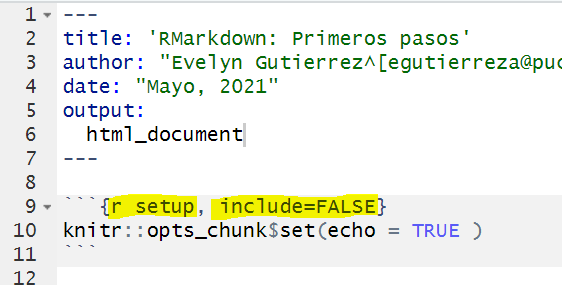
\includegraphics[width=0.4\textwidth,height=\textheight]{images/global.png}

\hypertarget{configuraciuxf3n-de-chunks}{%
\subsection{Configuración de chunks}\label{configuraciuxf3n-de-chunks}}

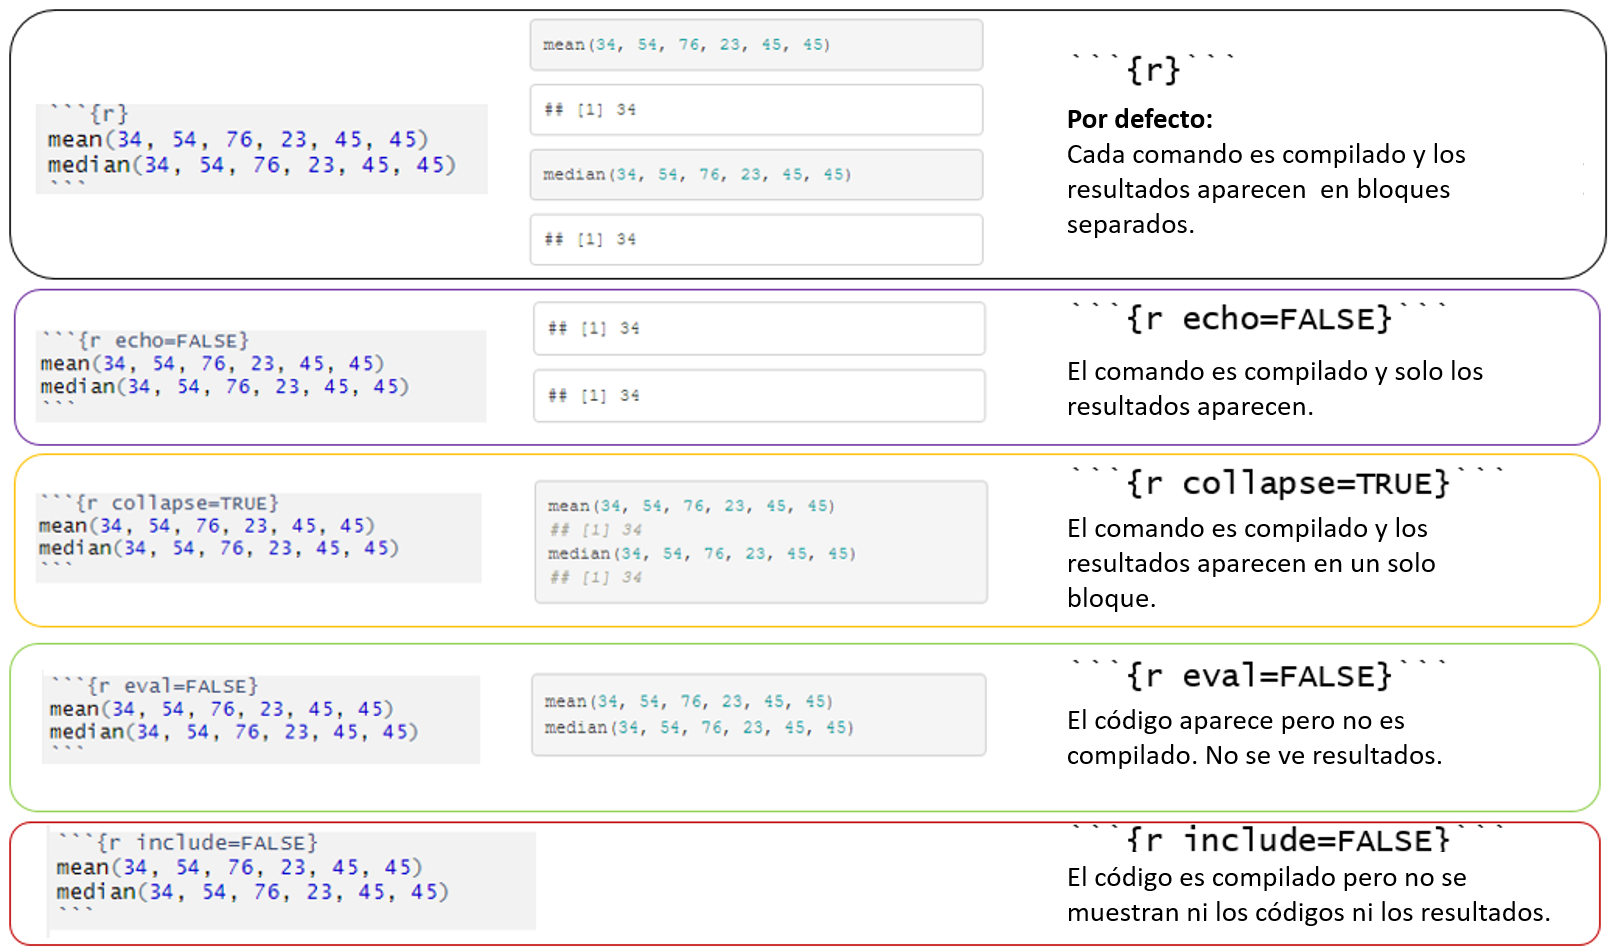
\includegraphics[width=0.7\textwidth,height=\textheight]{images/chunks.png}

\hypertarget{otros-detalles}{%
\subsection{Otros detalles:}\label{otros-detalles}}

\begin{itemize}
\item
  Es mejor añadir una línea en blanco entre diferentes elementos, como
  un título y un párrafo.
\item
  Para hacer un salto de línea: termine la línea con dos espacios +
  Enter.
\item
  Para añadir espacios adicionales entre líneas/secciones, utilice la
  etiqueta html: \texttt{\textless{}br\textgreater{}}.
\item
  Para incluir comentarios que no saldrán en el documento final, utilice
  comentarios en html:
  \texttt{\textless{}!-\/-\ Esto\ es\ un\ comentario\ -\/-\textgreater{}}.
\end{itemize}

\hypertarget{ejercicio.}{%
\subsection{Ejercicio. 👩‍💻 👨‍💻}\label{ejercicio.}}

\begin{itemize}
\tightlist
\item
  Crear un reporte de exploración y análisis de datos a partir de
  Rmarkdown. El reporte puede estar en html, pdf o word.

  \begin{itemize}
  \tightlist
  \item
    Utilizar la base de datos de interés o esta base de datos sobre el
    \href{/datos/breast-cancer.data}{cancer}. Obtenido del repositorio
    \href{https://archive.ics.uci.edu/ml/datasets/Breast+Cancer+Wisconsin+(Diagnostic)}{UCI
    Machine Learning repository}.
  \item
    Utilizar negritas y cursivas para resaltar los resultados del
    análisis.
  \item
    Utilizar secciones para dividir el análisis de los datos. Ejemplo:
    sección lectura de datos, sección de exploración y sección de
    regresión.
  \item
    Utilizar expresiones matemáticas en Rmd para mostrar la formula de
    alguna de las medidas de resumen que vaya a utilizar en el análisis.
  \item
    Utilizar chunks con códigos de R. - Pu
  \end{itemize}
\end{itemize}

\textbf{Ejemplo:}

\begin{itemize}
\tightlist
\item
  Reporte en
  \href{https://github.com/VilmaRomero/R-Ladies-Lima-rmarkdown/raw/master/reporte/Censo.pdf}{pdf}
  realizado por \href{https://vilmaromero.github.io/}{Vilma Romero
  (RLadies Lima)}. El códido fuente está disponible en
  \href{https://github.com/VilmaRomero/R-Ladies-Lima-rmarkdown/blob/master/reporte/Censo.Rmd}{github}.
\item
  \href{datos/Cap_100_Infraestructura\%202017.sav}{Datos del censo}
\end{itemize}

\hypertarget{muxe1s-sobre-rmarkdown}{%
\section{Más sobre Rmarkdown:}\label{muxe1s-sobre-rmarkdown}}

\textbf{Siguiente sesión:} \href{personalizar.html}{Personalizar Rmd}

\hypertarget{muxe1s-recursos}{%
\subsection{Más recursos}\label{muxe1s-recursos}}

\begin{itemize}
\item
  Yihui Xie, J. J. Allaire, Garrett Grolemund, 2020-10-14,
  \href{https://bookdown.org/yihui/rmarkdown/}{R Markdown: The
  Definitive Guide}
\item
  Yihui Xie, Christophe Dervieux, Emily Riederer, 2020-09-21,
  \href{https://bookdown.org/yihui/rmarkdown-cookbook/}{R Markdown
  Cookbook}
\item
  Yihui Xie, \href{https://yihui.org/knitr/}{knitr. Elegant, flexible,
  and fast dynamic report generation with R}
\item
  \href{https://rstudio.com/resources/cheatsheets/}{Rmarkdown et RStudio
  Cheatsheets}
\item
  RStudio, \href{https://rmarkdown.rstudio.com/gallery.HTML}{RMarkdown
  Gallery}
\item
  \href{https://www.markdowntutorial.com/}{Markdown Tutorial}
\item
  Karl Broman,
  \href{http://kbroman.org/Tools4RR/assets/lectures/03_knitr_Rmd_withnotes.pdf}{Writing
  reproducible reports. knitr with R Markdown}
\item
  Michael Clark, 2019-11-06,
  \href{https://m-clark.github.io/Introduction-to-Rmarkdown/}{Introduction
  to R Markdown}
\item
  Yan Holtz, 10 December 2018,
  \href{https://holtzy.github.io/Pimp-my-rmd/}{Pimp my RMD: a few tips
  for R Markdown}
\item
  Alison Hill · Desirée De Leon,
  \href{https://rstudio-education.github.io/sharing-short-notice/\#1}{Sharing
  on Short Notice. HOW TO GET YOUR TEACHING MATERIALS ONLINE WITH R
  MARKDOWN}
\item
  \href{http://www.geo.uzh.ch/microsite/reproducible_research/post/rr-r-publication/}{Writing
  publications with R}, Wed, Aug 17, 2016
\item
  Mike Frank \& Chris Hartgerink, 2017-07-31,
  \href{https://libscie.github.io/rmarkdown-workshop/handout.html\#headers-tables-and-graphs}{RMarkdown
  for writing reproducible scientific papers}
\item
  Marian L. Schmidt, May 11th, 2016,
  \href{https://rpubs.com/marschmi/RMarkdown}{Creating Dynamic Documents
  with RMarkdown and Knitr}
\item
  Thea Knowles, January 14, 2020,
  \href{https://rpubs.com/thealk/academic-writing}{RMarkdown and
  Bookdown for Academic Writing in R}
\end{itemize}

\hypertarget{compartir-documentos-en-luxednea}{%
\subsection{Compartir documentos en
línea:}\label{compartir-documentos-en-luxednea}}

\begin{itemize}
\tightlist
\item
  \href{https://rpubs.com/}{RPubs}
\item
  \href{https://app.netlify.com/drop}{Netlify}
\item
  \href{https://resources.github.com/whitepapers/github-and-rstudio/}{Github}
\end{itemize}

\end{document}
